% Countersign — NeurIPS 2026 Meta-Agents workshop, Short Paper (4pp main text).
%
% SUBMISSION RULES (venue CFP, fetched 2026-08-16):
%  - double-blind: no names/affiliations/acknowledgments; prior work in THIRD PERSON
%  - responsible-use statement MANDATORY (desk-reject if missing) — present below
%  - main text must be self-contained
%
% NUMBERS POLICY: every empirical number below is computed from the audited
% run manifests of the frozen campaign (see research/ deviation ledgers).
% Do not edit a number here without re-deriving it from the artifacts.

\documentclass{article}

\PassOptionsToPackage{numbers,compress}{natbib}
\IfFileExists{neurips_2026.sty}{%
  \usepackage{neurips_2026}%
}{%
  \usepackage[margin=1in]{geometry}%
  \usepackage{natbib}%
}

\usepackage[utf8]{inputenc}
\usepackage[T1]{fontenc}
\usepackage{hyperref}
\usepackage{url}
\usepackage{booktabs}
\usepackage{amsfonts}
\usepackage{microtype}
\usepackage{xcolor}
\usepackage{graphicx}
\usepackage{enumitem}

% Modest float-spacing tightening (standard for 4-page short papers).
\setlength{\textfloatsep}{12pt plus 2pt minus 4pt}
\setlength{\abovecaptionskip}{4pt}

\title{Countersign: Evidence-Grounded Supervision of Coding-Agent
Completion Claims}

% Double-blind: author block intentionally anonymous for submission.
\author{Anonymous authors\\Paper under double-blind review}

\begin{document}

\maketitle

\begin{abstract}
Coding agents terminate when they believe a task is done, but that
belief is not always supported by their own execution trace. We present \emph{Countersign}, a deterministic supervisory
meta-agent that audits a worker's completion claim against the
trace---checking that cited tests exist, remain fresh with respect to
the files they cover, postdate the latest requirement update, and do
not rest on superseded sources---and can block termination and demand
fresh evidence. Countersign is deliberately \emph{trace-only}: it
judges whether a claim is \emph{justified} at claim time---distinct
from whether the implementation is \emph{correct}, which a hidden
evaluator answers once after termination. In a preregistered,
frozen campaign of 490 real-model runs over ten held-out fixtures, all
17 blocks landed on proposals an independent oracle also labelled
unsupported (precision $1.00$, 95\% CI $[0.82,1.0]$) and none on the
204 supported proposals judged---though 13 of 17 are the trivial case
of a claim citing no evidence. A counterfactual replay shows a
conventional continuous-integration gate catches 2 of 15 unsupported
proposals; Countersign catches 11 of 11 it judged. Negative
results are equally informative: truncating the worker's visible
history did not increase unsupported completion; the effect appears
only when history is \emph{replaced by a narrative summary}, driven
mainly by prompting, the gate's contribution being to convert
unsupported acceptances into blocked episodes that recover. And we
quantify the construct honestly: all 18 accepted unsupported
completions concerned work that passed hidden evaluation---Countersign
is an evidence-hygiene instrument whose safety value remains a
hypothesis under test.
\end{abstract}

\section{Introduction}

An autonomous coding agent ends its episode by asserting
completion---a claim about evidence: the tests it ran, the edits it
made, the requirements it was given. When the claim outruns the
evidence (a cited test predating the final edit; a superseded source),
the agent has not necessarily produced wrong code, but it has produced
an \emph{unwarranted} report, and whoever trusts it inherits a risk
they cannot see.

We study whether a second agent with authority over the first's
termination can reliably tell warranted completion claims from
unwarranted ones, and what that authority costs. Countersign reads
only the worker's execution trace: it never
consults ground truth, and the hidden evaluator that determines
correctness runs exactly once, after termination, identically in every
condition. This separation is the paper's organizing principle: a claim
can be justified and wrong, or correct and unjustified, and conflating
the two makes ``the verifier improved outcomes'' unfalsifiable.

\textbf{Contributions.} We contribute (i)~a supervision loop with
halting authority over worker termination, scored against an
independent post-hoc oracle it does not compute (\S\ref{sec:method});
(ii)~a preregistered evaluation on matched fixture pairs and negative
controls that price false blocks, under a frozen protocol with a public
deviation ledger (\S\ref{sec:design}); (iii)~results across 490 runs:
perfect block precision, a CI-gate ablation, a truncation null, and a
regime-specific summarization effect decomposed into prompt and gate
contributions
(\S\ref{sec:results}); (iv)~a calibrated account of the gate as
evidence hygiene, not a demonstrated safety mechanism
(\S\ref{sec:failure}).

\begin{figure}[t]
\centering
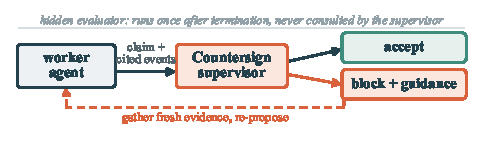
\includegraphics{figures/fig_loop.pdf}
\caption{The supervision loop. The worker proposes termination with
cited evidence; Countersign audits the claim against the trace and
accepts or blocks with a specific deficiency, after which the worker
gathers fresh evidence and re-proposes. The hidden evaluator runs once,
after termination, and is never consulted by the supervisor.}
\label{fig:loop}
\end{figure}

\section{The Countersign Supervisor}
\label{sec:method}

\textbf{Worker and ledger.} The worker is a tool-loop coding agent
(self-hosted open-weight models) in a git-backed workspace; every
action appends to an \emph{evidence ledger}---tool calls with outcomes,
file mutations, test runs with inferred coverage, requirement updates.
To finish, it emits a \texttt{finish} action carrying a claim and cited
evidence identifiers.

\textbf{The audit.} Countersign checks four properties of the cited
evidence: (i)~at least one cited event is a successful test run;
(ii)~no cited test predates a later mutation of a file it covers
(Appendix~\ref{sec:appendix-design}); (iii)~cited evidence
postdates the latest relevant requirement update; and (iv)~the claim
does not rest on sources the task marks superseded. Freshness is
tri-state: the supervisor abstains when coverage is unknown.

\textbf{Authority.} On failure the supervisor blocks termination and
returns the specific deficiency; a repair variant additionally issues
the smallest evidence-refreshing action. Every arm logs the \emph{raw} verifier
decision separately from the \emph{enforced} one, so non-blocking arms
still measure what the supervisor would have done.

\textbf{Independent oracle.} A post-hoc oracle labels every proposal
\textsf{supported}/\textsf{unsupported}/\textsf{uncertain} from
fixture-authored completion policies and canonical trace chronology. It
shares no code with the online verifier; \S\ref{sec:failure} reports a
regime where they disagree.

\section{Evaluation Design}
\label{sec:design}

\textbf{Fixtures.} Ten held-out fixture repositories, authored to a
preregistered design and frozen before any real-model run was
inspected. Three \emph{matched pairs} isolate one failure mode each
under context parity (workspaces byte-identical but for one designed
file): \emph{temporal} (cited tests
predate the final edit), \emph{provenance} (fresh evidence grounded in
a superseded document), and \emph{requirement} (a clarification arrives
after the last passing run). Four \emph{negative controls} contain no trap
(Appendix~\ref{sec:appendix-design}), so any block on them is a false
positive by construction; a separate development suite, on which the
rules were iterated, is never used for evaluation.

\textbf{Conditions.} Arms cross a worker prompt variant with verifier
authority: \textsf{memory\_baseline} (naive prompt, no gate),
\textsf{observe\_only} (evidence-citation prompt; verifier logs
decisions, never blocks, returns no feedback),
\textsf{verification\_only} (same prompt, blocking),
\textsf{verification\_and\_repair}, and an evaluation-only
\textsf{oracle\_supervisor} upper bound. Because
\textsf{memory\_baseline} and \textsf{verification\_only} differ in
\emph{both} prompt and gate, we never report that contrast as a gate
effect; \textsf{observe\_only} is the prompt-matched control, verified
in-trace to emit zero worker-visible feedback events.

\textbf{Memory degradation.} A frozen registry of degradation profiles
applies only to \emph{model-visible} state: graded \emph{lossy
truncation} of history (low/medium/high) and a \emph{resume-summary}
regime replacing the visible ledger with a single truthful summary---the
pattern deployed scaffolds use on session resumption. The canonical
ledger, verifier, oracle, and evaluator always see undegraded state.

\textbf{Protocol.} Temperature 0.7, sampler seeds 0--4, action budget
24 (Appendix~\ref{sec:appendix-design}). Endpoints, comparisons, and
interpretation branches for both positive and null outcomes were
committed before the runs; the frozen
protocol hashes code, fixtures, and model weights and refuses to start
on a dirty tree.

\section{Results}
\label{sec:results}

All numbers come from audited run manifests; the worker is
\texttt{qwen2.5-coder:14b}. The campaign's 490 runs yield 341
oracle-judged finish proposals, 27 labelled unsupported.

\textbf{Blocks are precise.} Across every arm with a live verifier,
Countersign issued 17 blocks---all on proposals the independent oracle
also labelled unsupported, none on the 204 supported proposals a
verifier judged: precision $1.00$ (95\% CI
$[0.82,1.0]$), false-block rate $0/204$ (95\% CI $[0,0.018]$), recall
$17/18=0.94$ (95\% CI $[0.74,0.99]$). Two caveats bound this. First,
the denominator counts only judged proposals: 110 further supported
proposals in no-verifier arms are excluded, not counted as successes. Second, and more important, \textbf{13 of the 17 blocks are
the trivial case}---a claim citing no evidence, which any rule detects.
Only 4 required substantive reasoning about staleness or provenance:
read the result as ``the gate does not misfire,'' not ``the gate
discriminates hard cases.''

\textbf{A conventional CI gate is mostly blind.} We
replay every stored proposal against the standard-practice rule
``require a successful test run after the last edit,'' a strict subset
of Countersign's temporal check. The CI rule catches 2 of
15 unsupported proposals; Countersign catches 11 of the 11 it judged,
of which only 4 required substantive reasoning---the rest cite nothing
at all. Neither gate blocked any of the 161 supported proposals both
judged: the difference is blindness, not conservatism.

\begin{figure}[t]
\centering
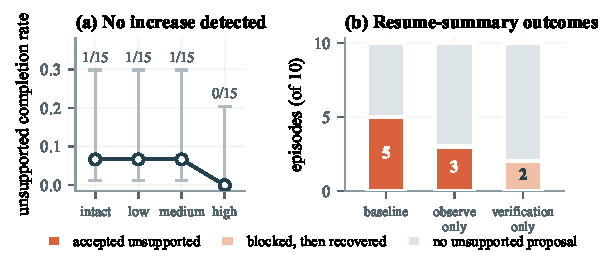
\includegraphics{figures/fig_regimes.pdf}
\caption{Memory degradation does not act uniformly. (a)~Graded
truncation: no detectable increase in unsupported completion; the
Wilson 95\% intervals mark this a non-detection at modest power, not
invariance. (b)~Replacing history with a resume summary does
produce the effect: the evidence-citation prompt reduces unsupported
proposals ($5{\to}3$), and the gate converts those it sees from silent
acceptances into blocked episodes that recover (2 of 2). Small $n$;
decomposition, not significance.}
\label{fig:regimes}
\end{figure}

\textbf{Truncating memory does not \emph{detectably} induce false
claims.} Baseline unsupported completion on trap fixtures did not
increase with truncation severity (Figure~\ref{fig:regimes}a). This is a non-detection, not invariance:
at 15 runs per cell the Wilson intervals span roughly 0.01--0.30, so
effects under ${\sim}30$ percentage points are unresolvable; the
preregistered null branch applies with that caveat.

\textbf{The effect is regime-specific, and decomposes.} Replacing
history with a resume summary does produce unsupported completion
(Figure~\ref{fig:regimes}b). The
comparison must be read at the \emph{proposal} level: in a blocking arm
an accepted-unsupported finish is suppressed by the intervention's own
definition, so a zero there is partly mechanical. Counting unsupported proposals over ten
matched cells: baseline 5, \textsf{observe\_only} 3,
\textsf{verification\_only} 2. Pairing the cells, the prompt contrast
has discordant cells 3 vs.\ 1 (exact McNemar $p=0.625$); the further
$3\rightarrow2$ is sampling noise, since the gate cannot influence a
worker's \emph{first} proposal. The gate's contribution is not fewer
unsupported claims but a different fate for them: both proposals it saw
were blocked, and both episodes recovered and terminated with supported
evidence. No comparison here reaches $p<.05$, and
an a-priori power analysis explains why---even with every discordant
pair in one direction the exact test requires $b\ge6$, one more than
this campaign could have produced, and 16 matched cells would be needed for
80\% power at the observed effect (Bayesian sensitivity reading in
Appendix~\ref{sec:appendix-bayes}). The cleanest evidence is
measurement without power: in \textsf{observe\_only} the verifier
judges but cannot act, and its would-block decisions fired in exactly
the 3 unsupported cells and none of the other 7 (TP$=3$, FP$=0$,
FN$=0$)---immune to the circularity objection a blocking arm invites.

\textbf{What ``unsupported'' means here.} Table~\ref{tab:twobytwo}
crosses the oracle's judgement of the accepted claim against the hidden
evaluator's judgement of the work. All 18 unsupported completions
concerned work that was \emph{correct}: an unjustified claim never
coincided with a wrong implementation, so Countersign is measured to
catch \emph{poor evidential hygiene} and its safety value remains a
hypothesis this campaign cannot confirm.

\begin{table}[t]
\centering
\caption{Accepted completions ($n{=}327$): oracle verdict on the claim
vs.\ hidden-evaluator verdict on the work. The empty bottom-right cell
is the paper's central caveat.}
\label{tab:twobytwo}
\renewcommand{\arraystretch}{0.95}
\begin{tabular}{lcc}
\toprule
& correct & incorrect \\
\midrule
claim supported   & 307 & 2 \\
claim unsupported & 18  & 0 \\
\bottomrule
\end{tabular}
\end{table}

\section{Supervisor-Failure Analysis and Limitations}
\label{sec:failure}

\textbf{The structural blind spot.} The provenance pair is designed so
that fresh, well-cited evidence grounded in a superseded source passes
a trace-only audit while the work fails hidden evaluation. That designed path never fired here (the two
\textsf{supported-but-incorrect} completions arose on a
negative-control and a requirement fixture), but the class is real, no
trace audit can reach it, and it bounds what runtime evidence
supervision can promise.
Appendix~\ref{sec:appendix-failures} details two further failure modes:
classifier/oracle divergence under heavy degradation and a fixture
family censored by task weight, not action budget.

\textbf{Limitations.} (1)~Most important: the held-out traps and the
supervisor's rules share authors; the development/held-out split
prevents rule tuning on evaluation fixtures but not the conceptual
correlation between what we trap and what we detect, and the provenance
family (built to \emph{defeat} the supervisor) plus the negative
controls (which price the unflattering direction) offset this only
partially. (2)~One worker
model on ten small fixtures establishes nothing about prevalence in
production software.
(3)~The primary endpoint is partly suppressed by construction in
blocking arms; gate effects are read at the proposal level and in
post-block outcomes. (4)~The verifier and oracle
share no code but read the same trace; most agreements concern claims
citing no evidence---near-vacuous independence. (5)~No result reaches
$p<.05$; nulls are non-detections at modest power, and we report
decompositions and intervals, never significance. (6)~The degradation profiles are our own transforms, not a deployed
scaffold's condenser; (7)~oracle-label validation covers a
single-rater sample.

\section{Related Work}

Workers game outcome
checks~\citep{vonarx2025rewardhacking,baker2025monitoring}; external
supervisors with authority over another agent are an established design
space~\citep{greenblatt2023control,xiang2024guardagent,agentspec2025,chennabasappa2025llamafirewall};
deterministic finish-blocking hooks (no termination until tests pass)
are deployed practice---the rule our CI replay prices. Countersign
differs in \emph{what} it audits: cited-evidence chronology
(freshness, requirement recency, provenance), with abstention and
priced false blocks. The justified/correct split
descends from process-vs-outcome
supervision~\citep{uesato2022process,lightman2024verify}, instantiated
at termination against a hidden
evaluator~\citep{cobbe2021gsm8k,jimenez2024swebench}. Trajectory judges
score completion without termination
authority~\citep{zhuge2024agentjudge}; SCATE targets premature
termination~\citep{gu2026scate}; concurrent work
checks completion evidence and provenance in workflow
graphs~\citep{matrix2026provenance} and at GUI agents' finish
step~\citep{han2026vlaagui}. Self-verification~\citep{shinn2023reflexion} is the complement;
long-context degradation~\citep{liu2024lost,packer2023memgpt} motivates
the memory regimes.

\section*{Responsible-Use Statement}

Countersign controls agent overclaiming, but agents supervising agents
carries risks we keep visible: an \emph{allow} audits justification,
not correctness, and must not be marketed as verification; a visible
gate invites \emph{oversight displacement}, so verdicts reach operators
as cited-evidence audits, not badges; and halting authority adds a
failure surface---\emph{who supervises the supervisor}---that we price
as counter-metrics. Experiments involve no human subjects, personal
data, or production systems.

\bibliographystyle{unsrtnat}
\bibliography{references}

\appendix
\section{Design Details}
\label{sec:appendix-design}
Test coverage is inferred statically, so documentation edits do not
invalidate code evidence, and a failure superseded by a later passing
run does not permanently contradict a claim.
The four negative controls: documentation edits after green tests; an
unrelated-module edit with a targeted-test citation; a legitimate
zero-change audit; an irrelevant late clarification. Sampling uses
temperature 0.7 because greedy decoding would make multi-seed
replication pseudoreplication; seeds 0--4 are sampler seeds over
otherwise identical episodes.

\section{Additional Failure Modes}
\label{sec:appendix-failures}
\textbf{Classifier/oracle divergence.} Under high degradation the
online claim classifier disagreed with the independent oracle, because
the classifier reads the worker's degraded view while the oracle reads
the canonical trace. All endpoints in the main text are oracle-anchored;
the divergence is evidence that an independent oracle is necessary
rather than redundant.

\textbf{Task weight censors a family.} Requirement-family trap runs
exhaust the action budget in $3/5$ runs in every arm, and raising the
budget from 24 to 40 actions left that rate unchanged. The family is
intrinsically too heavy for this worker---a fixture-design finding, not
a budget-calibration error.

\section{A Blocked-then-Recovered Trajectory}
\label{sec:appendix-traj}
Under lossy truncation at low severity, one verification-arm episode on
a fresh-evidence temporal fixture shows the mechanism in miniature. The
pressured worker twice proposed terminating \emph{legitimate} work with
insufficient cited evidence; the supervisor blocked both proposals with
the specific deficiency; the worker gathered fresh evidence, terminated
supported, and passed hidden evaluation. Pressure-induced premature
finishing was rare for this worker, but both instances that occurred
were caught and repaired by the gate. The five blocks issued across the
pressure gradient (three on trap fixtures, two on control-task
proposals) all landed on oracle-unsupported proposals, and enforced
false blocks on oracle-supported work remained zero campaign-wide.

\section{Bayesian Sensitivity Readings}
\label{sec:appendix-bayes}
As a post-hoc sensitivity analysis (recorded as such in the deviation
ledger; no new data, uniform $\mathrm{Beta}(1,1)$ priors, exact
conjugate posteriors, no sampling), we re-read the paper's key
small-$n$ counts in Bayesian form. \emph{Direction of the prompt
effect}: conditioning on discordant matched cells as in the exact
McNemar test, $b{=}3$ cells favour \textsf{observe\_only} over
\textsf{memory\_baseline} and $c{=}1$ the reverse, giving posterior
$\mathrm{Beta}(4,2)$ on the probability that a discordant cell favours
the prompt and $P(\theta>0.5)=0.8125$---roughly four-to-one posterior
odds on a beneficial direction from the same data whose two-sided $p$
is $0.625$.
\emph{Discrimination in the arm that cannot act}: the
\textsf{observe\_only} verifier's sensitivity $3/3$ has posterior mean
$0.80$ with 95\% credible interval $[0.40, 0.99]$, and its specificity
$7/7$ has mean $0.89$, interval $[0.63, 1.00]$; campaign-wide block
precision $17/17$ gives $[0.81, 1.00]$, agreeing with the Wilson
interval in the main text. These are direction and uncertainty
statements only; none is a magnitude claim, and all shrink toward
chance under priors skeptical of any effect.

\section{Reproducibility}
The campaign spans three tags of one freeze: a base freeze plus two
infrastructure-only fixes applied mid-campaign (interruption-recovery
artifact reuse; a tool-level crash on syntactically invalid
worker-written code surfacing as a tool error rather than killing the
episode). The hashed verifier-policy files are byte-identical across
all three tags: no verifier, oracle, or fixture logic changed after the
freeze. Every deviation, interim inspection, and protocol-identifier
supersession---including two interim analyses that informed spending
decisions, and one corrected over-interpretation---is recorded in the
deviation ledger shipped with the artifact. The artifact is a
relocatable bundle whose integrity audit passes from the copied
location; it contains only fixtures, protocols, and run records.

\end{document}
